\documentclass[../../main.tex]{subfiles}

\begin{document}

\section{Experimento 3: 45 períodos observados, 5 de dependencia}
Aquí redujimos aún más la cantidad de períodos de dependencia, pasando de 10 a 5,
pero esta vez con 0 subidas. Esto implica que la proporción de períodos de dependencia
sobre observados es de 0.11, pero la tendencia modelada en ellos es monótona decreciente,
como se observa en la Figura \ref{fig:time_series_exp3}.

\begin{figure}[H]
    \centering
    \begin{minipage}{0.48\textwidth}
        \centering
        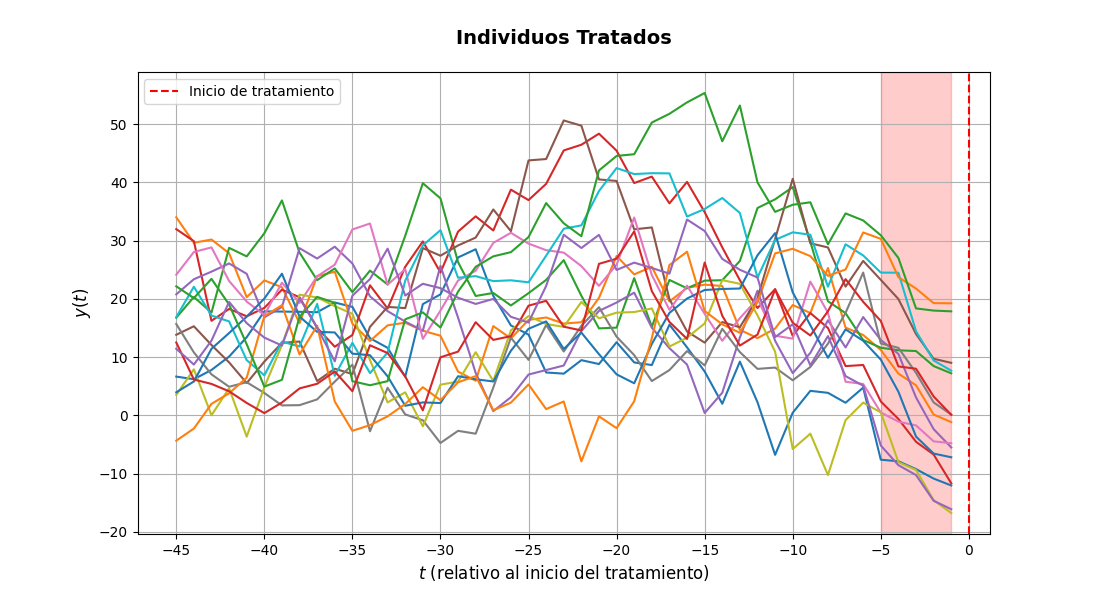
\includegraphics[scale=0.3]{figs/Exp3/plot_time_series_Tratados.png}
    \end{minipage}
    \hfill
    \begin{minipage}{0.48\textwidth}
        \centering
        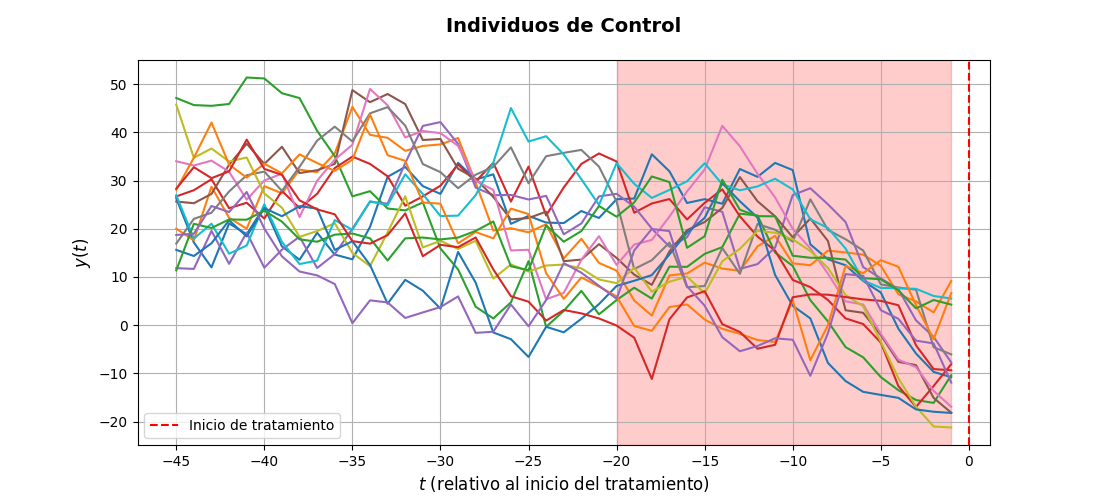
\includegraphics[scale=0.3]{figs/Exp3/plot_time_series_de_Control.png}
    \end{minipage}
    \vspace{0.5em}
    \begin{minipage}{0.6\textwidth}
        \centering
        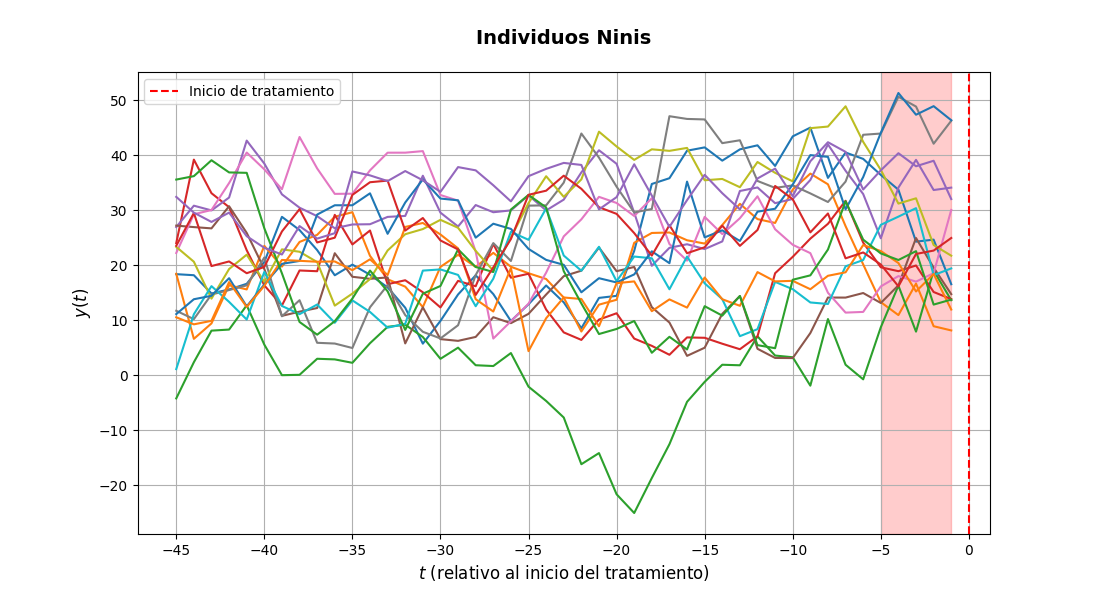
\includegraphics[scale=0.3]{figs/Exp3/plot_time_series_Ninis.png}
    \end{minipage}
    \caption{Ejemplos de series de tiempo generadas para cada grupo en el Experimento 3.
    Los períodos con un fondo rojo indican los períodos de dependencia para tratados y
    controles, en donde se ve el comportamiento monótono decreciente. La línea
    punteada roja indica el inicio de tratamiento para cada individuo.}
    \label{fig:time_series_exp3}
\end{figure}

La Tabla \ref{tab:results_exp3} muestra los valores obtenidos de las diferentes métricas.
Para nuestra sorpresa, en el caso de las redes, fueron mejores que los obtenidos en el
Experimento 1, en donde teníamos la misma cantidad de períodos observados, de los cuales
casi la mitad mostraban un compartamiento decreciente con ruido. Esto puede indicar que
sacarle las subidas a los períodos de dependencia, lo cual disminuye la complejidad del
patrón a hallar, favorece en gran medida a las arquitecturas de redes neuronales. Sin
embargo, el PSM presentó un rendimiento menor al visto en dicho escenario, contrario a
nuestra hipótesis.

\begin{table}[H]
    \centering
    \renewcommand{\arraystretch}{1.2}
    \begin{tabular}{|c|c|c|c|}
        \hline
         & \textbf{Puntaje} \(F_1\) & \textbf{Precisión} & \textbf{Sensibilidad} \\ \hline\hline
        \textbf{LSTM}
            & 0.8257 & 0.727401 & 0.956803 \\ \hline
        \textbf{Convolucional}
            & 0.846412 & 0.750914 & \textbf{0.971327} \\ \hline
        \textbf{LSTM + Convolucional}
            & \textbf{0.84759} & \textbf{0.753195} & 0.970398 \\ \hline
        \textbf{PSM}
            & 0.533242 & 0.533978 & 0.532512 \\
        \hline
    \end{tabular}
    \caption{Promedio de las métricas \(F_1\), precisión y sensibilidad sobre la
    clase positiva (controles) en el conjunto de test en las 100 simulaciones del
    Experimento 3.}
    \label{tab:results_exp3}
\end{table}

En la Tabla \ref{tab:hyperparams_exp3} se reflejan los resultados correspondientes
a los hiperparámetros, en donde nuevamente se observa lo mismo que antes.

\begin{table}[H]
    \centering
    \renewcommand{\arraystretch}{1.2}
    \begin{tabular}{|c|c|c|c|c|}
        \hline
            & \makecell{\textbf{Tamaño}\\\textbf{de lote}}
            & \makecell{\textbf{Neuronas en}\\\textbf{capas ocultas}}
            & \makecell{\textbf{Tasa de}\\\textbf{aprendizaje}}
            & \textbf{Dropout} \\ \hline\hline
        \textbf{LSTM}
            & 64 (35\%) & 128 (57\%) & 0.001 (100\%) & 0.3 (64\%) \\ \hline
        \textbf{Convolucional}
            & 32 (42\%) & -          & 0.001 (89\%)  & 0.3 (76\%) \\ \hline
        \makecell{\textbf{LSTM +}\\\textbf{Convolucional}}
            & 32 (50\%) & 32 (35\%), 64 (35\%) & 0.001 (87\%) & 0.3 (71\%) \\
        \hline
    \end{tabular}
    \caption{Valores de hiperparámetros seleccionados con mayor frecuencia en las 100
    simulaciones en cada arquitectura. Cada celda contiene dicho valor y entre paréntesis
    el porcentaje de simulaciones en el resultó ser el mejor, de acuerdo a la optimización
    realizada por Optuna mediante validación cruzada.}
    \label{tab:hyperparams_exp3}
\end{table}

\end{document}